\documentclass[fontsize=12pt]{scrartcl}
\usepackage[ngerman]{babel}
\usepackage[utf8]{inputenc}
%\usepackage[latin1]{inputenc}
\usepackage{amsmath}
\usepackage{amstext}
\usepackage{amssymb}
\usepackage{stmaryrd}
\usepackage{verbatim}
\usepackage{mathrsfs}
\usepackage{extarrows}
\usepackage[arrow, matrix, curve]{xy}
\usepackage[centering,includeheadfoot,margin=2cm]{geometry}
\usepackage{gensymb}
\usepackage{graphicx}
\usepackage{framed}
\usepackage{xcolor}
\usepackage{float}
\usepackage{graphicx} 
\usepackage{sidecap}
\usepackage{blindtext,wrapfig}
\usepackage{epstopdf}
\usepackage{import}
\usepackage{fancyhdr}
\usepackage{fancybox}
\usepackage{paralist}
\usepackage{graphicx}
\usepackage{caption}
\usepackage{subcaption}
\renewcommand{\l}{\left\vert}
\renewcommand{\r}{\right\vert}
\DeclareGraphicsRule{.tif}{png}{.png}{`convert #1 `basename #1 .tif`.png} 
\pagestyle{fancy}
\fancyhf{}
\fancyhead[R]{Physikalisches Praktikum 1}
\fancyhead[L]{Linda Werneck, Gentian Rrafshi}
\fancyfoot[R]{\thepage}
\fancyfoot[L]{\today}

\begin{document}

\begin{minipage}{\textwidth}
\begin{center}\large
\title{ O20 Brechungsindexbestimmung mit dem Prismen-Spektralapparat \\
		~\\
		~\\
		Assistent: Lukas Schwarz \\
		Datum Versuchsdurchführung: \\
		03.06.2015}

\author{bearbeitet von\\
		Gruppe 3-031: \\
		Linda Werneck Matrnr. 2901495 \\
		Gentian Rrafshi Matrnr. 2721617 }
\date{\today}

\maketitle

\end{center}
\end{minipage}

\newpage

\tableofcontents

\newpage
\noindent

\section{ Versuchsziel}

In diesem Versuch sollen wir die Abhängigkeit von Brechungsindex zu Wellenlänge und die Dispersion bestimmen.

\section{ Grundlagen}

Zwischen 380\,nm bis 780\,nm ist das vom menschlichen Auge sichtbare Licht. Das Sneulliussche-Brechungsgesetz
\begin{equation*}
\frac{\sin(\alpha)}{\sin(\beta)} = \frac{c_1}{c_2} = \frac{n_2}{n_1}
\end{equation*}
\noindent
beschreibt die Brechung von Licht, welches von einem Medium ins andere Medium fällt. Hierbei ist $n_i$ der relative Brechungsindex des jeweiligen 
Mediums und $\alpha$ ist der Einfallswinkel sowie $\beta$ der Ausfallswinkel.\\
~\\
Im Vakuum gilt für den Brechungsindex $n=1$, weswegen:
\begin{equation*}
\frac{\sin(\alpha)}{\sin(\beta)} = \frac{c_{\text{vak}}}{c_2} = n
\end{equation*}
\noindent
Hier ist $n$ nun absolute Brechungsindex. Als Eselsbrücke kann man sich hierbei also merken, dass für $n_1 > n_2$ erfolgt die Brechung weg vom Lot und 
$n_1 < n_2$ erfolgt zum Lot hin.\\
~\\
Ist der Ausfallswinkel $\beta \geq \frac{\pi}{2}$, so liegt Totalreflexion vom optisch dichteren ins optisch dünnerer Medium. Dabei entsteht eine Grenzwinkel $\alpha_T$, welcher gegeben ist durch.
\begin{equation*}
\sin(\alpha) = \sin(\alpha_T) = \frac{n_2}{n_1}
\end{equation*}
Will man den Brechungsindex eines Materials bestimmen, so kann man dies mit Hilfe eines Prismas in dem selben Material und des Prismen-Spektralapparats 
dies messen bzw. bestimmen. Das Prinzip des Prismenspektralapparats ist die spektrale Zerlegung des Lichtes mit Hilfe eines Dispersionsprismas erfolgt. 
Der Prismen-Spektralapparat besteht aus einem Kollimator, einem Prismentisch, einem Fernrohr sowie einer Lampe. Fällt Licht auf das Prisma, so macht das 
Kollimator das Licht parallel. Durch das Fernrohr kann man durch verstellen in einem bestimmten Winkel die Spektrallinien des einfallenden Lichts sehen. 
Durch verstellen erhält man dann die minimale Ablenkung $\delta_{\text{min}}$. Damit ist der Brechungsindex durch folgende Formel berechenbar:
\begin{equation*}
n=\frac{\sin(\frac{\delta_{\text{min}}+\varphi}{2})}{\sin(\frac{\varphi}{2})}
\end{equation*}
\noindent
Wobei $\varphi$ der brechende Winkel ist, welcher nichts anderes als der Winkel gegenüber der Hypotenuse des Prismendreiecks ist.
\newpage

\section{Versuchsaufbau und Durchführung}

\begin{figure}[h]
\begin{minipage}{0.5\textwidth}
\centering
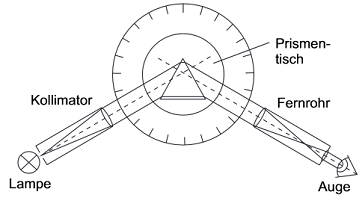
\includegraphics[scale=0.75]{Graphik/O20-1}
\caption{Versuchsaufbau$^{\cite{A}}$}
\end{minipage}
\begin{minipage}{0.5\textwidth}
\centering
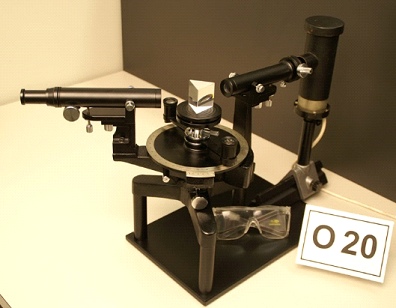
\includegraphics[scale=0.5]{Graphik/Versuchsaufbau}
\caption{Versuchsaufbau$^{\cite{A}}$}
\end{minipage}
\end{figure}
\noindent
Bevor mit den Messungen begonnen werden kann, muss man den Prismen-Spektralapparat in die Richtige Voreinstellung bringen. Dazu schwenkt man das Fernrohr so, dass man damit direkt in den Kollimator hinein sehen kann. Bei beleuchtetem Spalt wird mit dem Okular die schärfe des Bildes und des Fadenkreuzes eingestellt.

\subsection{Bestimmung des brechenden Winkels $\varphi$}
Das Prisma wird auf dem Prismentisch so ausgerichtet, dass die Spitze des Prismas mit dem brechenden Winkel in Richtung des Kollimators zeigt. Das Licht wird angemacht. Mit dem Fernrohr sucht man die beiden reflektierten weißen Lichtstrahlen $\varphi_{\text{links}}, \varphi_{\text{rechts}}$ und notiert deren Position in Grad.
\begin{figure}[h]
\centering
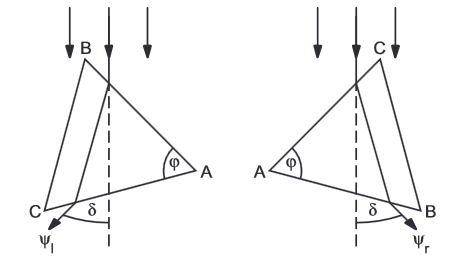
\includegraphics[scale=1]{Graphik/O20-4}
\caption{Versuchsskizze$^{\cite{A}}$}
\end{figure}
\newpage
\noindent
\subsection{Messung der minimalen Ablenkwinkel}
Der minimale Ablenkwinkel wird für die mittlere Wellenlänge bestimmt, also für die gelbe Spektrallinie. Dazu stellt man das Prisma mittenzentriert so auf den Prismentisch wie in Abbildung 3. Das Tischchen wird so gedreht, dass die Ablenkung des gelben Strahls kleiner wird. Das Fernrohr wird immer so mitgedreht, dass man Sicht auf die Spektrallinien hat. Wenn man das Tischchen so weit dreht, dass die Bewegung der Strahlen trotz gleicher Drehrichtung des Tisches die Ablenkungsrichtung der Strahlen ändert, hat man die Stelle des minimalen Ablenkwinkels gefunden. Das Prisma darf ab dann nicht mehr bewegt werden und man kann mit der Messung beginnen.
Gemessen wird die Ablenkung der Spektrallinien in Grad. Dazu dreht man das Fernrohr so, dass sich das Fadenkreuz in der Mitte der zu messenden Spektrallinie befindet und liest an der Haupt- und Nonius-Skala den Ablenkungswinkel $\delta_{\text{min}}$ ab. Diese Messung wiederholt man für alle sichtbaren Spektrallinien.
Danach wird das Prisma so hingelegt, wie in  Abbildung 3 zu sehen ist. Man stellt nach demselben Schema den minimalen Ablenkwinkel ein und misst wieder alle sichtbaren Spektrallinien.

\section{Formeln}

\subsection{Formel für Brechungswinkel}
\begin{equation}
\label{phi}
\varphi=\frac{\l \phi_{\text{links}} - \phi_{\text{rechts}}\r}{2}
\end{equation}
$\varphi$: Brechender Winkel, $\phi_{\text{links}}$ bzw.$ \phi_{\text{rechts}}$: linker und rechter reflektierter Strahl aus \textbf{3.1}

\subsection{Formel für den minimalen Ablenkwinkel}
\begin{equation}
\label{delta}
\delta_{\text{min}}=\frac{\l\delta_{\text{links}} - \delta_{\text{rechts}}\r}{2}
\end{equation}
$\delta_{\text{min}}$: minimaler Ablenkwinkel, $\delta_{\text{links}}$, $\delta_{\text{rechts}}$: Auslenkung nach links und rechts

\subsection{Formel für Brechungsindex}
\begin{equation}
\label{n}
n=\frac{\sin(\frac{\delta_{\text{min}}+\varphi}{2})}{\sin(\frac{\varphi}{2})}
\end{equation}
$n$: Brechungsindex

\subsection{Formel für Auflösungsvermögen}
\begin{equation}
\label{n}
A=b\cdot\l \frac{\partial n}{\partial \lambda} \r
\end{equation}
$n$: Brechungsindex; $\lambda$: Wellenlänge; $b=3$\,cm: Breite der Prismen.

\newpage

\section{ Messwerte}
\begin{figure}[h]
\centering
\caption{Messwerte Prisma 1}
\begin{tabular}{|c|c|c|} \hline
&										$[^{\circ}]$ &	[Rad] \\ \hline
$\phi_{\text{links}}$&			136,67	&2,38		\\ \hline
$\phi_{\text{rechts}}$&		17,00	  &0,30		\\ \hline
$\varphi$	&59,83	&1,04\\ \hline
\end{tabular} \\
\begin{tabular}{|c|c|c|c|} \hline
Wellenlänge [nm] & Farbe & $\psi_{\text{rechts}}$ $[^{\circ}]$ & $\psi_{\text{links}}$ $[^{\circ}]$  \\ \hline
671,00	&Rot		&122,50	&45,33	\\ \hline
579,00	&Gelb		&122,67	&45,17	\\ \hline
546,10	&grün		&122,83	&45,00	\\ \hline
491,60	&dunkelgrün	&123,00	&44,83	\\ \hline
435,80	&blau		&123,17	&44,33	\\ \hline
404,70	&violett	&124,08	&44,00	\\ \hline
\end{tabular} \\
\end{figure}

\begin{figure}[h]
\centering
\caption{Messwerte Prisma 2}
\begin{tabular}{|c|c|c|} \hline
&							$[^{\circ}]$ &	[Rad] \\ \hline
$\phi_{\text{links}}$&		134,67		&2,34		\\ \hline
$\phi_{\text{rechts}}$&		14,83	  	&0,26		\\ \hline
$\varphi$		&			59,75		&1,04\\ \hline
\end{tabular} \\
\begin{tabular}{|c|c|c|c|} \hline
Wellenlänge [nm] & Farbe & $\psi_{\text{rechts}}$ $[^{\circ}]$ & $\psi_{\text{links}}$ $[^{\circ}]$  \\ \hline
671,00	&Rot		&131,83	&12,00	\\ \hline
579,00	&Gelb		&132,25	&12,08	\\ \hline
546,10	&grün		&132,58	&12,33	\\ \hline
404,70	&violett	&135,83	&14,17	\\ \hline
\end{tabular} \\
\end{figure}
Die Original Messwerte befinden sich im Anhang.
\newpage

\section{ Auswertung}

\subsection{Berechnung des brechenden Winkels $\varphi$}

Zuallererst soll der Brechungswinkel $\varphi$ berechnet werden. Dies geschieht mit Hilfe von Formel (\ref{phi}). Daraus ergibt sich für die Prismen:
\begin{align*}
\varphi_{\text{Prisma 1}} &=\frac{\l \phi_l - \phi_r  \r}{2} = \frac{\l 136,67^{\circ} - 17^{\circ}  \r}{2} = 59,83^{\circ} \\
~\\
\varphi_{\text{Prisma 2}} &=\frac{\l \phi_l - \phi_r  \r}{2} = \frac{\l 134,33^{\circ} - 14,83^{\circ}  \r}{2} = 59,75^{\circ}
\end{align*}\\

Da unsere Prismen gleichseitige Dreiecke sind, sollten die Winkel $60^{\circ}$ sein. 

\subsection{Berechnung des minimalen Ablenkwinkels $\delta_{\text{min}}$}

In diesem Teil der Auswertung soll die minimale Ablenkung $\delta_{\text{min}}$ für verschieden Wellenlängen berechnet werden. Beispielhaft wird hier beim ersten Prisma die minimale Ablenkung für rotes Lichts errechnet:
\begin{align*}
\delta_{\text{min}} &=\frac{\l \psi_l - \psi_r  \r}{2} = \frac{\l 122,50^{\circ} - 45,33^{\circ}  \r}{2} = 38,58^{\circ}
\end{align*}\\
Die weiteren Ergebnisse werden in der nachfolgenden Tabelle ausgeführt:
\begin{figure}[h]
\centering
\caption{Ergebnisse Prisma 1}
\begin{tabular}{|c|c|c|c|} \hline
Wellenlänge [nm] & $\psi_{\text{rechts}}$ $[^{\circ}]$ & $\psi_{\text{links}}$ $[^{\circ}]$ & $\delta_{\text{min}}$ $[^{\circ}]$ \\ \hline
671,00	&122,50	&45,33	&38,58\\ \hline
579,00	&122,67	&45,17	&38,75\\ \hline
546,10	&122,83	&45,00	&38,92\\ \hline
491,60	&123,00	&44,83	&39,08\\ \hline
435,80	&123,17	&44,33	&39,42\\ \hline
404,70	&124,08	&44,00	&40,04\\ \hline
\end{tabular} \\
\end{figure}
\begin{figure}[h]
\centering
\caption{Ergebnisse Prisma 2}
\begin{tabular}{|c|c|c|c|} \hline
Wellenlänge [nm] & $\psi_{\text{rechts}}$ $[^{\circ}]$ & $\psi_{\text{links}}$ $[^{\circ}]$ & $\delta_{\text{min}}$ $[^{\circ}]$ \\ \hline
671,00	&131,83	&12,00	&59,92\\ \hline
579,00	&132,25	&12,08	&60,08\\ \hline
546,10	&132,58	&12,33	&60,13\\ \hline
404,70	&135,83	&14,17	&60,58\\ \hline
\end{tabular} \\
\end{figure}
\newpage
\subsection{Brechungsindex}

Ziel des Versuchs ist es den Brechungsindex in Abhängigkeit zur Wellenlänge zu bestimmen.
Mit Hilfe von $\delta_{\text{min}}$ und $\varphi$ und Formel (\ref{n}) können wir nun den Brechungsindex für die verschiedenen Wellenlängen ausrechnen, hier als Beispiel für rotes Licht beim ersten Prisma.
\begin{align*}
n=\frac{\sin(\frac{\delta_{\text{min}} + \varphi}{2 })}{\sin( \frac{\varphi}{2})} =\frac{\sin(\frac{38,58^{\circ} + 59,63^{\circ}}{2 })}{\sin( \frac{59,63^{\circ}}{2})} = 1,5181
\end{align*}
Die anderen Werte werden tabellarisch dargestellt:	
\begin{figure}[h]
\centering
\caption{Ergebnisse Prisma 1}
\begin{tabular}{|c|c|c|c|c|} \hline
Wellenlänge [nm] & $\psi_{\text{rechts}}$ $[^{\circ}]$ & $\psi_{\text{links}}$ $[^{\circ}]$ & $\delta_{\text{min}}$ $[^{\circ}]$ & n \\ \hline
671,00	&122,50	&45,33	&38,58	&1,5181 \\ \hline
579,00	&122,67	&45,17	&38,75	&1,5200\\ \hline
546,10	&122,83	&45,00	&38,92	&1,5219\\ \hline
491,60	&123,00	&44,83	&39,08	&1,5238\\ \hline
435,80	&123,17	&44,33	&39,42	&1,5276\\ \hline
404,70	&124,08	&44,00	&40,04	&1,5347\\ \hline
\end{tabular} \\
\end{figure}
\begin{figure}[h]
\centering
\caption{Ergebnisse Prisma 2}
\begin{tabular}{|c|c|c|c|c|} \hline
Wellenlänge [nm] & $\psi_{\text{rechts}}$ $[^{\circ}]$ & $\psi_{\text{links}}$ $[^{\circ}]$ & $\delta_{\text{min}}$ $[^{\circ}]$ & n  \\ \hline
671,00	&131,83	&12,00	&59,92	&1,7360\\ \hline
579,00	&132,25	&12,08	&60,08	&1,7374\\ \hline
546,10	&132,58	&12,33	&60,13	&1,7378\\ \hline
404,70	&135,83	&14,17	&60,58	&1,7418\\ \hline
\end{tabular} \\
\end{figure}\\
\noindent
Angesichts dieser Brechungsindizes, erhalten wir, dass das erste Prisma vermutlich Kronglas$^{\cite{2}}$ und das zweite Prisma könnte Flintglas$^{\cite{3}}$sein.
\newpage
\noindent
Im Anschluss werden für beide Prismen Brechungsindex-Wellenlänge-Diagramme erstellt:
\begin{figure}[h]
\centering
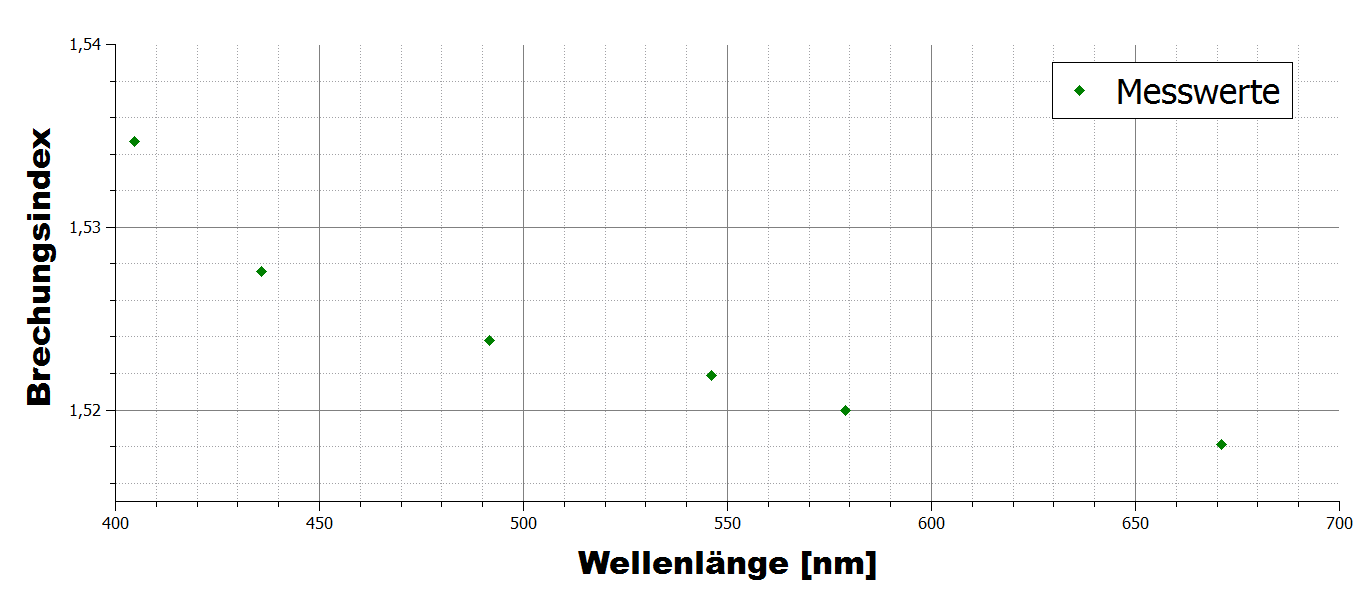
\includegraphics[scale=0.4]{Graphik/Prisma1}
\caption{Brechungsindex-Wellenlänge-Diagramm für Prisma 1}
\end{figure}
\begin{figure}[h]
\centering
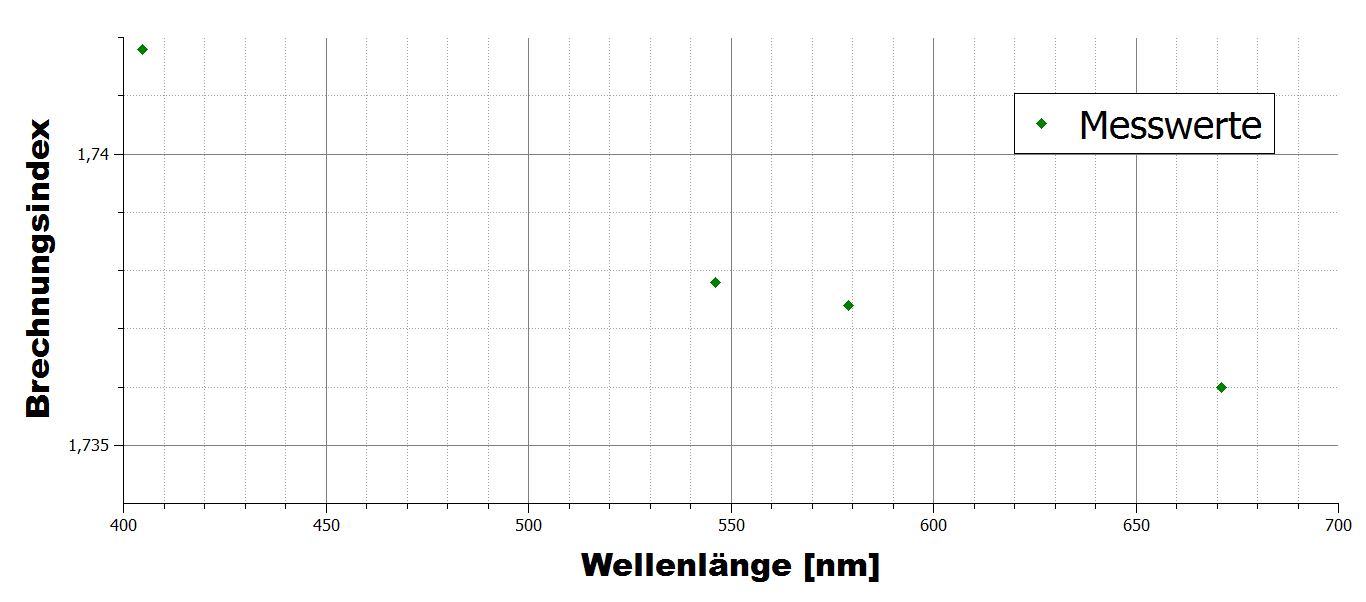
\includegraphics[scale=0.4]{Graphik/Prisma2}
\caption{Brechungsindex-Wellenlänge-Diagramm für Prisma 2 }
\end{figure}
\newpage
\noindent
Fitten wir linear die Punkte für Wellenlänge 671\,nm und 579\,nm, so erhalten wir eine jeweils eine Geradenfunktionen. Setzen wir in diesen Funktionen die Wellenlänge 598\,nm, so erhalten wir für die Brechung der Na-D folgende Brechungsindizes:\\
\begin{center}
Prisma 1: 	n= 1,51979 \\
Prisma 2:	n= 1,73724
\end{center}

\subsection{Auflösungsvermögen}

Mit der Formel (4) können wir das Auflösungsvermögen berechnen. Dabei ist $b=3\text{cm}=0,03\text{m}$.	
Für die Berechnung von $\l \frac{\partial n}{\partial \lambda} \r$ benutzen wir Qti-Plot. Wir liesen jeweils die zwei ersten Punkte und die zwei letzten Punkte von unseren Diagrammen linear Fitten und erhielten dann folgende Steigungen:
\begin{figure}[h]
\centering
\caption{Ergebnisse Prisma 2}
\begin{tabular}{|c|c|c|} \hline
 & Steigung ersten Zwei Punkte & Steigung letzten zwei Punkte   \\ \hline
Prisma 1 &	$-2,065\cdot 10^{4}$ $\frac{1}{\text{m}}$	&	$-2,283\cdot 10^{5}$ $\frac{1}{\text{m}}$	\\ \hline
Prisma 2 &	$-1,522\cdot 10^{4}$ $\frac{1}{\text{m}}$	&	$-2,829\cdot 10^{4}$ $\frac{1}{\text{m}}$	\\ \hline
\end{tabular} \\
\end{figure}\\
\noindent
Dadurch ergibt sich für unsere Auflösungsvermögen:
\begin{align*}
A _1&=0,03\text{m}\cdot\l -2,065\cdot 10^{4} \frac{1}{\text{m}}  \r = 6.195\cdot 10^{2}\\
A_2&=0,03\text{m}\cdot\l -1,522\cdot 10^{4} \frac{1}{\text{m}} \r = 4,566\cdot 10^{2}\\
A_3&=0,03\text{m}\cdot\l -2,283\cdot 10^{5} \frac{1}{\text{m}} \r = 6,849\cdot 10^{3}\\
A_4&=0,03\text{m}\cdot\l -2,829\cdot 10^{4} \frac{1}{\text{m}} \r = 8,487\cdot 10^{2}
\end{align*}
\newpage

\section{Fehlerquellen}

In diesem Versuch gab es im Grunde nur eine Fehlerquelle, das menschliche Auge. Daher wird als einzige 
Messungenauigkeit für $\Delta \delta_{\text{min}}=\Delta \varphi=0,1^{\circ}$ angenommen.\\
~\\
$\Delta n$ erhalten wir durch Fehlerfortpflanzung, wobei wir hier wieder für das rote Licht des ersten Prismas eine Beispielrechnung durchführen.
\begin{align*}
\Delta n &= \l \frac{\partial n}{\partial \varphi} \r \cdot \Delta \varphi + \l \frac{\partial n}{\partial \delta_{\text{min}}} \r \cdot \Delta\delta \\
&= \l \frac{\cos(\frac{\varphi + \delta}{2}) \cdot \sin({\frac{\varphi}{2}}) - \sin(\frac{\varphi + \delta}{2}) \cos(\frac{\varphi}{2})}{2\cdot 
\sin^2(\frac{\varphi}{2})}\r \cdot \Delta\varphi + \l \frac{\cos(\frac{\delta +\varphi}{2})}{2\cdot \sin(\frac{\varphi}{2})} \r  \cdot \Delta\delta\\
%
&= \l \frac{\cos(\frac{1,043759259 + 0,673064815}{2}) \sin({\frac{1,043759259}{2}}) - \sin(\frac{1,043759259 + 0,673064815}{2}) \cos(\frac{1,043759259}{2})}{2\cdot \sin^2(\frac{1,043759259}{2})}\r \cdot 0,00174
 \\
&+ \l \frac{\cos(\frac{0,673064815+1,043759259}{2})}{2\cdot \sin(\frac{1,043759259}{2})} \r  \cdot 0,00174
 \\
&= \l 0,002019664
 \r + \l 0,001143646
 \r = 0,00316
\end{align*}
\noindent
Für die anderen Werte ergibt sich:
\begin{figure}[h]
\begin{minipage}{0.5\textwidth}
\centering
\caption{Ergebnisse Prisma 1}
\begin{tabular}{|c|c|c|c|c|} \hline
Wellenlänge [nm]  & n & $\Delta n$ \\ \hline
671,00 &1,5181 &0,00316
\\ \hline
579,00	&1,5200 &0,00318
\\ \hline
546,10	&1,5219 &0,00319
\\ \hline
491,60	&1,5238 &0,00320
\\ \hline
435,80	&1,5276 &0,00323
\\ \hline
404,70	&1,5347 &0,00328
\\ \hline
\end{tabular} \\
\end{minipage}
\begin{minipage}{0.5\textwidth}
\vspace{-30pt}
\centering
\caption{Ergebnisse Prisma 2}
\begin{tabular}{|c|c|c|c|c|} \hline
Wellenlänge [nm] &  n & $\Delta n$  \\ \hline
671,00	&1,7360 &0,00438
\\ \hline
579,00	&1,7374 &0,00438
\\ \hline
546,10	&1,7378 &0,00439
\\ \hline
404,70	&1,7418 &0,00438
\\ \hline
\end{tabular} \\
\end{minipage}
\end{figure}

Unser Fehler werden in den folgenden zwei Diagrammen als Fehlerbalken dargestellt:
\newpage
\begin{figure}[H]
\centering
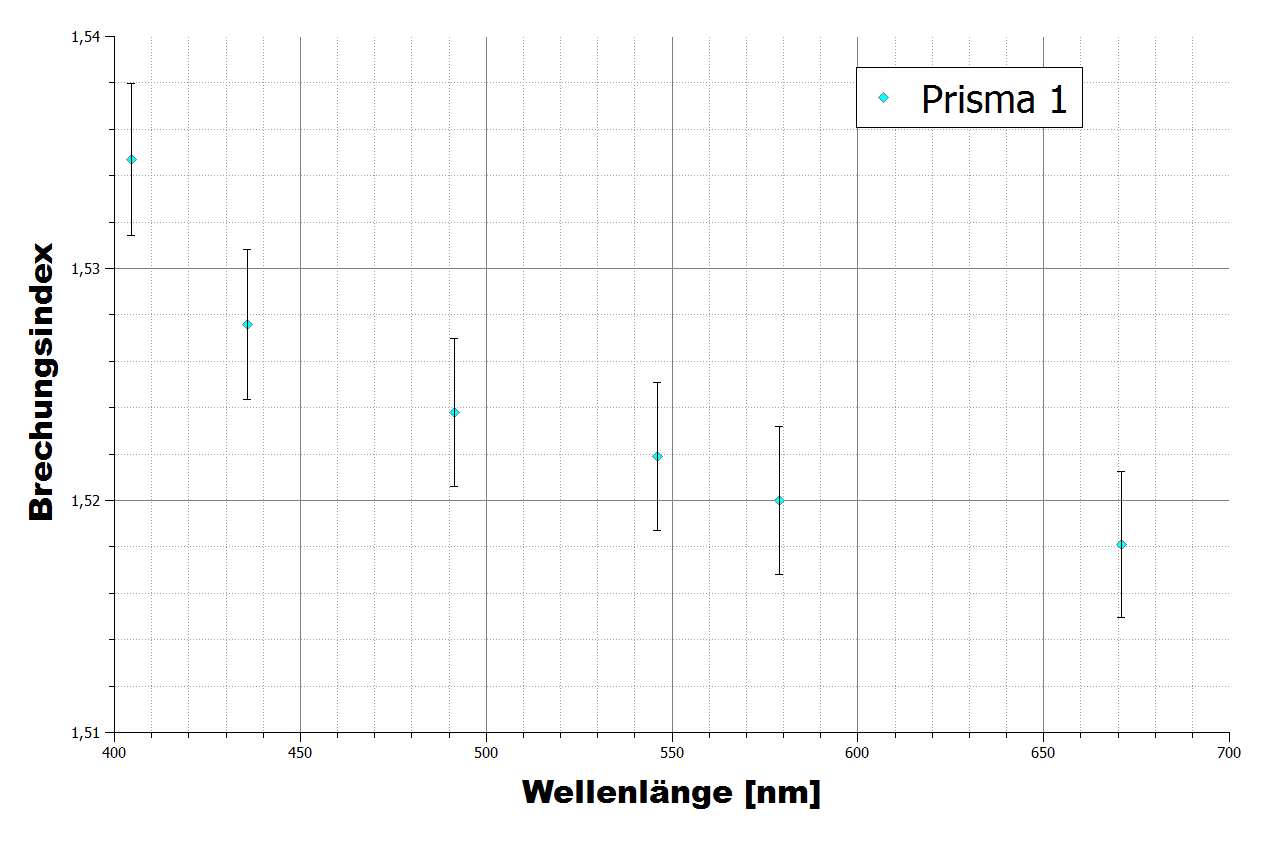
\includegraphics[scale=0.45]{Graphik/Prisma1Fehler}
\caption{Brechungsindex-Wellenlänge-Diagramm für Prisma 1}
\end{figure}
\begin{figure}[H]
\vspace{-25pt}
\centering
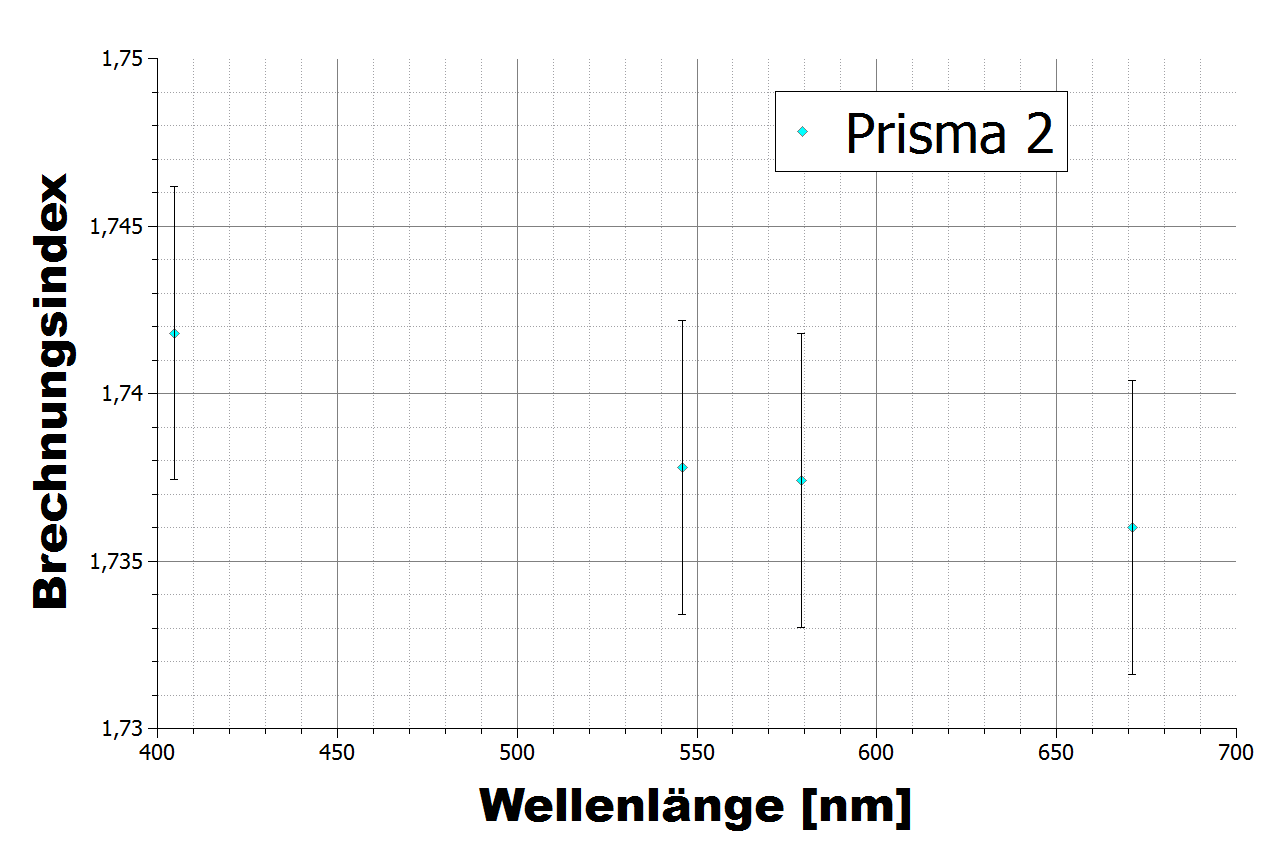
\includegraphics[scale=0.45]{Graphik/Prisma2Fehler}
\caption{Brechungsindex-Wellenlänge-Diagramm für Prisma 2 }
\end{figure}
\newpage

\section{Zusammenfassung}

Ziel des Versuchs war es den Brechungsindex beider Prismen für verschiedene Wellenlängen zu bestimmen, wir erhielten: 
\begin{figure}[h]
\begin{minipage}{0.5\textwidth}
\centering
\caption{Ergebnisse Prisma 1}
\begin{tabular}{|c|c|c|c|c|} \hline
Wellenlänge [nm]  & n & $\Delta n$ \\ \hline
671,00 &1,5181 &0,00316
\\ \hline
579,00	&1,5200 &0,00318
\\ \hline
546,10	&1,5219 &0,00319
\\ \hline
491,60	&1,5238 &0,00320
\\ \hline
435,80	&1,5276 &0,00323
\\ \hline
404,70	&1,5347 &0,00328
\\ \hline
\end{tabular} \\
\end{minipage}
\begin{minipage}{0.5\textwidth}
\vspace{-30pt}
\centering
\caption{Ergebnisse Prisma 2}
\begin{tabular}{|c|c|c|c|c|} \hline
Wellenlänge [nm] &  n & $\Delta n$  \\ \hline
671,00	&1,7360 &0,00438
\\ \hline
579,00	&1,7374 &0,00438
\\ \hline
546,10	&1,7378 &0,00439
\\ \hline
404,70	&1,7418 &0,00438
\\ \hline
\end{tabular} \\
\end{minipage}
\end{figure}

\noindent
Daraus erschließt sich für uns, dass es sich bei Prisma 1 um Kronglas und in Prisma 2 um Flintglas handelt. Desweiteren ergab sich durch lineares Fitten für die Na-D-Linie folgende Wellenlänge:
\begin{center}
Prisma 1: 	n= 1,51979 \\
Prisma 2:	n= 1,73724
\end{center}
\noindent
Durch weiteres Fitten und etwas rechen erhielten wir folgendes für die Auflösungsvermögen:
\begin{align*}
A _1&= 6.195\cdot 10^{2}\\
A_2&= 4,566\cdot 10^{2}\\
A_3&= 6,849\cdot 10^{3}\\
A_4&= 8,487\cdot 10^{2}
\end{align*}
\noindent

\newpage
\section{Literaturverzeichnis}

\renewcommand{\refname}{~}
\vspace{-30pt}
\begin{thebibliography}{xxxxxxxx}
	\bibitem[1]{1}		\textit{\glqq O20 Brechungsindexbestimmung mit dem Prismen-Spektralapparat\grqq , \\
								 in http:www3.physik.uni-stuttgart.de/studium/praktika/ap/},\\
								\textit{ unter http://www3.physik.uni-stuttgart.de/studium/praktika/ap/pdf\_dateien/O20.pdf abgerufen am 5.06.2015}
	\bibitem[2]{2}		\textit{	http://de.wikipedia.org/wiki/Kronglas abgerufen am 5.06.2015}
	\bibitem[3]{3}		\textit{	http://de.wikipedia.org/wiki/Flintglas abgerufen am 5.06.2015}
   \bibitem[A]{A}  	Graphik aus \textit{\glqq O20 Brechungsindexbestimmung mit dem Prismen-Spektralapparat\grqq , in 	\\
   								http://www3.physik.uni-stuttgart.de/studium/praktika/ap/}, \\
   								\textit{ unter 	http://www3.physik.uni-stuttgart.de/studium/praktika/ap/pdf\_dateienO20.pdf; abgerufen am 5.06.2015} 

\end{thebibliography}

\section{Anhang}

\end{document}